\documentclass[usenames, dvipsnames]{beamer}
%% Possible paper sizes: a0, a0b, a1, a2, a3, a4.
%% Possible orientations: portrait, landscape
%% Font sizes can be changed using the scale option.
\usepackage[size=a0,orientation=portrait,scale=1.59]{beamerposter}
\usepackage{xcolor}
\usetheme{LLT-poster}
\usecolortheme{Moris}

\usepackage[utf8]{inputenc}
\usepackage[T1]{fontenc}
\usepackage{graphicx}
\usepackage{booktabs}
\usepackage{lmodern}
\usepackage{hyperref}
\usepackage{amsmath}
\usepackage{amssymb}
\usetikzlibrary{arrows,shapes}

% For every picture that defines or uses external nodes, you'll have to
% apply the 'remember picture' style. To avoid some typing, we'll apply
% the style to all pictures.
\tikzstyle{every picture}+=[remember picture]
\tikzstyle{na} = [baseline=-.5ex]

% Neccessary since lmodern fonts declare only small math symbols
\DeclareFontShape{OMX}{cmex}{m}{n}{
  <-7.5> cmex7
  <7.5-8.5> cmex8
  <8.5-9.5> cmex9
  <9.5-> cmex10
}{}
\SetSymbolFont{largesymbols}{normal}{OMX}{cmex}{m}{n}
\SetSymbolFont{largesymbols}{bold}{OMX}{cmex}{m}{n}

\newcommand{\Losc}{\ensuremath{L^{\text{osc}}}}
\newcommand{\Lcoh}{\ensuremath{L^{\text{coh}}}}
\newcommand{\Ld}{\ensuremath{L^{\text{d}}}}
\newcommand{\Dm}{\ensuremath{\Delta m^2}}
\newcommand{\Important}{\textcolor{BrickRed}}
\newcommand{\Regular}{\textcolor{DeepBlue}}
\newcommand{\MidnightBlue}{\textcolor{MidnightBlue}}
\newcommand{\Orange}{\textcolor{Orange}}
\newcommand{\Maroon}{\textcolor{Maroon}}
\newcommand{\Bittersweet}{\textcolor{Bittersweet}}
\newcommand{\regitem}{\item[\Regular{$\bullet$}]}
\newcommand{\impitem}{\item[\Important{$\bullet$}]}
\newcommand{\midblitem}{\item[\MidnightBlue{$\bullet$}]}
\newcommand{\orangeitem}{\item[\Orange{$\bullet$}]}
\newcommand{\pineitem}{\item[\Maroon{$\bullet$}]}
\newcommand{\bitteritem}{\item[\Bittersweet{$\bullet$}]}
\newcommand{\sip}{\ensuremath{\sigma_p}}
\newcommand{\srel}{\ensuremath{\sigma_{\text{rel}}}}
\newcommand{\six}{\ensuremath{\sigma_x}}
\newcommand{\anue}{\ensuremath{\bar{\nu}_e}}

\author[]{\textbf{Konstantin Treskov} on behalf of the Daya Bay collaboration}
\title{Experimental study of decoherence effects\\ in neutrino oscillations in
Daya Bay}
\institute{Joint Institute for Nuclear Research, Dubna, Russia}

\begin{document}
\begin{frame}[fragile]
\begin{columns}[T]

%%%% First Column
    \hspace*{-2.5cm}
\begin{column}{.47\textwidth}
\begin{block}{Conventional neutrino oscillations}
\begin{itemize}
    \regitem Convetional approach to neutrino oscillations relies on a number of
        assumptions:
        \begin{itemize}
            \item Flavor state is a superposition of mass states with
                identical energies:
                \begin{equation*}
                    | \nu_\alpha \rangle = \sum_{i=1}^{3} V^*_{\alpha i}\, |
                    \nu_i(p) \rangle
                \end{equation*}
            \item Production and detection proccesses occur coherently.
            \item Mass states travel at speed of light.
        \end{itemize}
    \item That leads to extensively experimentally studied oscillation probability
    \begin{equation*}
        P_{\alpha\beta}(L) = \sum_{i,k=1}^3 V^*_{\alpha i} V_{\beta i}
        V^*_{\beta k}
        V_{\alpha k} \exp \left( - 2\pi i  \frac{L}{\Losc_{ik}}\right), \quad
        \ensuremath{\Losc_{ik} = \dfrac{4 \pi E}{\Dm_{ik}}}
    \end{equation*}
    \impitem There are internal inconsistencies within that approach:
        \begin{itemize}
            \item  Distance \ensuremath{L} can't be defined with delocalized
                states.
            \item The coherence of production and detection should be proven.
            \item Equal energy assumption is not Lorentz-invariant.
        \end{itemize}
\end{itemize}
\end{block}

\begin{block}{Neutrino oscillation with wave packets}
  \begin{itemize}
      \item The issues above can be addressed when one consider neutrino
          flavor state as coherent superposition of mass states with different
          momenta:
          \begin{equation*}
              \hspace*{-2cm} |\nu_i(k)\rangle \rightarrow  \int \frac{dk}{2\pi} f(k, p,
           \sigma^2) | \nu_i(k) \rangle
          \end{equation*}
      \item Assuming form factor is Gaussian the oscillation probability reads: 
          \colorbox{CornflowerBlue!15}{\raisebox{0}[1.1\height]{\makebox[27.3em]{
        \begin{equation*}
         \hspace*{-1cm}P_{\alpha\beta}(L) = \sum_{k,\,j=1}^3\frac{ V^{\phantom\dagger}_{k
                 \beta }V^*_{\alpha k}V^{\phantom\dagger}_{j \alpha }
                 V^*_{\beta j} }{\Maroon{\sqrt[4]{1 +
             \left(L/\Ld_{kj}\right)^2}}}\,\,
             \exp{\left[-\frac{\textcolor{MidnightBlue}{\left(L/\Lcoh_{kj}\right)^2}}{\Maroon{1+\left(L/\Ld_{kj}\right)^2}}
    -\textcolor{Orange}{\mathrm{D}^2_{kj}\right]}}
    \text{e}^{-i(\varphi_{kj} + \varphi^d_{kj})}
    \end{equation*}
     }}}
    \begin{equation*}
        \hspace*{-1cm} \varphi^\text{d}_{kj} =
        - \Maroon{\frac
        {L/L^\text{d}_{kj}}{1+\left(L/{L^\text{d}_{kj}}\right)^2}}
        \MidnightBlue{
        \left(\frac L {\Lcoh_{kj}}\right)^2}
        + \Maroon{\frac{1}{2} \arctan { \frac{L}{\Ld_{kj}}}}
    ,\quad \varphi_{kl}=2\pi\frac{L}{L^\text{osc}_{kj}}, \quad
    \end{equation*}
    \begin{itemize}
        \bitteritem \Bittersweet{$\sigma_{rel}=\sigma_{p}/p$} is a relative
            momentum dispersion of wave packet. \newline
            \Important{\ensuremath{\sigma_p}} is intrinsic
    momentum dispersion of wave packet. It depends on a kinematics of
    production and detection proccesses.\\ In this work
    \ensuremath{\sigma_p = \text{const}} is assumed.
    \midblitem \MidnightBlue{$\Lcoh = \frac{\Losc_{kj}}{\sqrt 2 
    \pi\sigma_\text{rel}}$} is a \MidnightBlue{coherence length}.
            At this distance separation of wave packets due to different group
            velocities suppresses interference between mass states.
        \pineitem \Maroon{$\Ld_{kj}  =
            \frac{\Lcoh_{kj}}{2\sqrt{2}\sigma_{\text{rel}}}$} is a
            \Maroon{dispersion length} of wave packet. At this distance
             coherence between mass states is partially restored due to
             spacial broadening of wave packet.
         \orangeitem \Orange{\ensuremath{ \text{D}^2_{kj} =\frac{1}{2} \left(
             \frac{\Dm_{kj}}{4 p^2\sigma_\text{rel}} \right)^2}} 
         suppresses the coherence of mass states due to spacial localization of production and
             detection regions.
    \end{itemize}
  \end{itemize}
\end{block}


\begin{block}{What do we know about \sip?}
    \begin{itemize}
        \item No fisrt principle QFT calculations.
        \item Only phenomenological estimates such as:
        \begin{itemize}
            \item $\sip \sim 1\, \text{MeV}, \,\, \six \sim 10^{-11}\, \text{cm}$
                --- uranium atom size;
            \item $\sip \sim 1-10 \, \text{keV}, \,\, \siz ~ 10^{-8} -
                10^{-7} \, \text{cm}$ --- atomic scale;
            \item $\sip \sim 0.1 \, \text{eV}, \,\, \siz ~ 10^{-4} \, \text{cm}$
                --- pressure broadening.
        \end{itemize}
        \impitem Lack of experimental studies.
    \end{itemize}
\end{block}

\begin{block}{Reference}
    \begin{columns}[T]
        \begin{column}{0.8\textwidth}
            \begin{itemize}
                \impitem \textbf{Study of the wave packet treatment of neutrino
                oscillation at Daya Bay},
                \\ Eur.Phys.J. C77 (2017) no.9, 606
            \end{itemize}
        \end{column}
        \begin{column}{0.2\textwidth}
        \vspace*{-3cm}
        \hspace*{\fill}
        \href{https://link.springer.com/article/10.1140%2Fepjc%2Fs10052-017-4970-y}
        { 
\includegraphics[scale=0.8]{./pics/paper_qr_nologo.png}}
        \end{column}
    \end{columns}
\end{block}
                
\end{column}

%%%% Second Column
\begin{column}{.47\textwidth}
    \linespread{1.01}
\begin{block}{Daya Bay setup}
    \vskip-.7cm
    \begin{columns}[T]
        \begin{column}{0.58\textwidth}
            \begin{itemize}
                \item \Important{8} detectors with 20 tons of
                    Gd-dopped liquid scintillator.
                \item \Important{6} nuclear reactors with 2.9 GW of thermal
                    power.
                \item \anue\, detection through IBD 
                    \hspace*{3.5cm}{\centering{\Important{$\anue + p \rightarrow e^+ + n$}}}
                \item Use coincidence of prompt and delayed signals in time to select
                    \anue\, events.
                \item \anue\, sample based on \Important{621} days:
                    \vskip1.5ex
                    {\centering
                    \begin{table*}
                        \renewcommand{\arraystretch}{1.2}
                        \begin{tabular}{@{}cccc{}@}
                            \toprule
                        & \Regular{EH1} & \Regular{EH2} & \Regular{EH3}\\
                            \Regular{Events}\,\,\, & \Important{613813}\, &
                            \Important{477144}\, & \Important{150255}
                            \bottomrule
                        \end{tabular}
                    \end{table*}}
                    \vskip1ex
                \item Energy resolution \ensuremath{\sim 8\,\%} at 1~MeV.
            \end{itemize}
        \end{column}
        \begin{column}{0.47\textwidth}
        \vspace*{-2.5cm}
            \begin{figure}[T]
                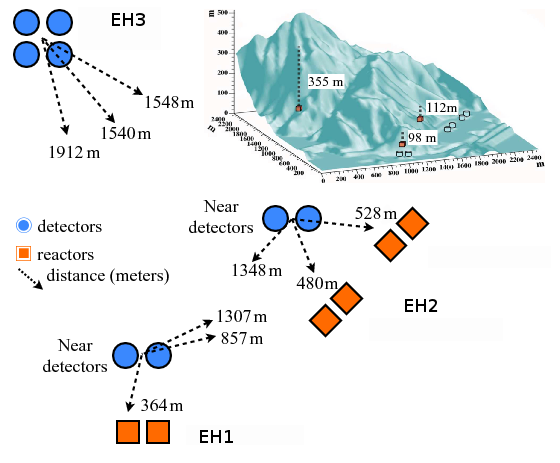
\includegraphics[scale=0.8]{./pics/DYBdiag_3.png}
            \end{figure}
            \begin{figure}[b]
                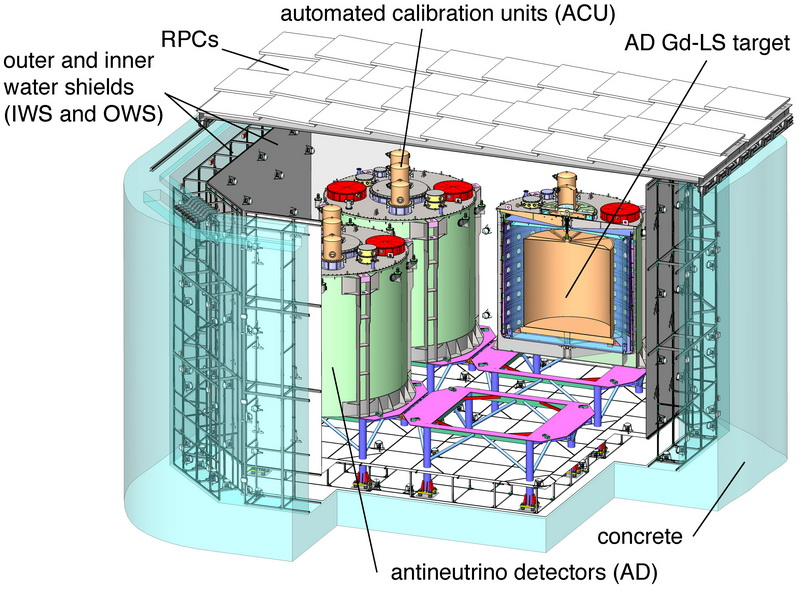
\includegraphics[scale=2.8]{./pics/Fig2_DYB_farhalllabel.png}
            \end{figure}
        \end{column}
    \end{columns}
\end{block}

\vspace{.3cm}
\begin{block}{Statistical method}
    \begin{columns}[T]
        \begin{column}{0.47\textwidth}
            \vspace*{-1cm}
            \begin{figure}
                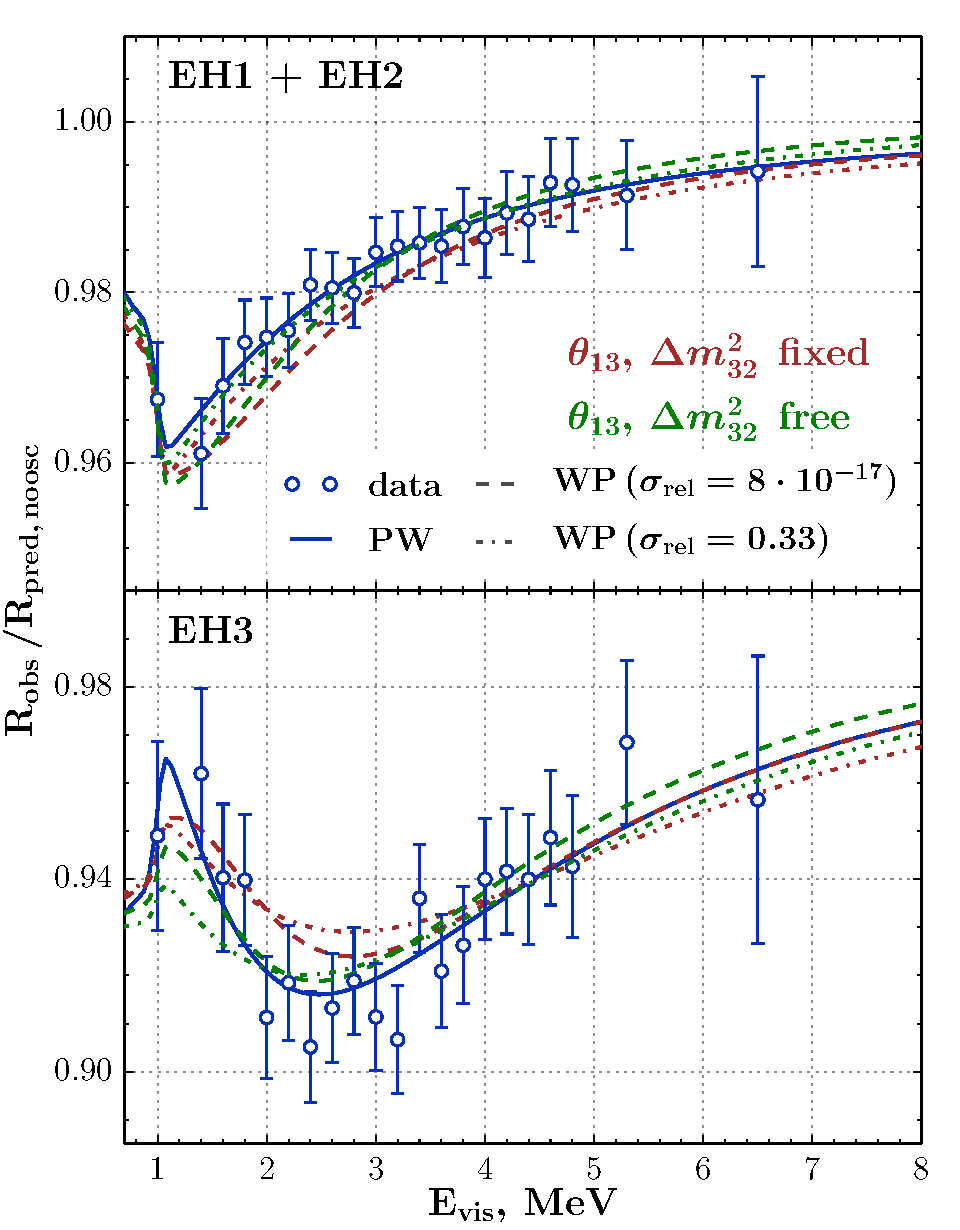
\includegraphics[scale=1.22]{./pics/EH-ratio_5sigma-s_double-EH_bold.pdf}
            \end{figure}
        \end{column}
        \hspace*{1.5cm}
        \begin{column}{0.5\textwidth}
              Test statistic is defined as:
                    \begin{equation*}
                        \chi^2 = (\mathbf{d} -
                            \mathbf{t} (\boldsymbol{\eta}))^T V^{-1}(\mathbf{d} -
                            \mathbf{t} (\boldsymbol{\eta}))
                    \end{equation*} 
            \vspace*{-1.85cm}
            {\hskip-1cm{
            \begin{itemize}
                \item Free parameters:
                    \begin{itemize}
                    \impitem \Important{\srel}
                    \impitem \Important{\ensuremath{\sin^2 2\theta_{13}}}
                    \impitem \Important{\ensuremath{\Dm_{32}}}
                    \impitem Flux normalization \Important{N}
                    \end{itemize}
                \item Systematical uncertainties are propagated via covariance
                    matrix \Important{V}
                    \impitem Confidence levels are constucted via \Important{fixed-level
                        \ensuremath{\Delta \chi^2}} and 
                        \Important{Feldman-Cousins} methods.
            \end{itemize}
        }
        }
        \end{column}
    \end{columns}
\end{block}

\vspace{.3cm}
\begin{block}{Results and Discussion}
    \begin{columns}[T]
        \begin{column}{0.42\textwidth}
            \begin{figure}[T]
                \hspace*{-0.7cm}
                % \vfill
                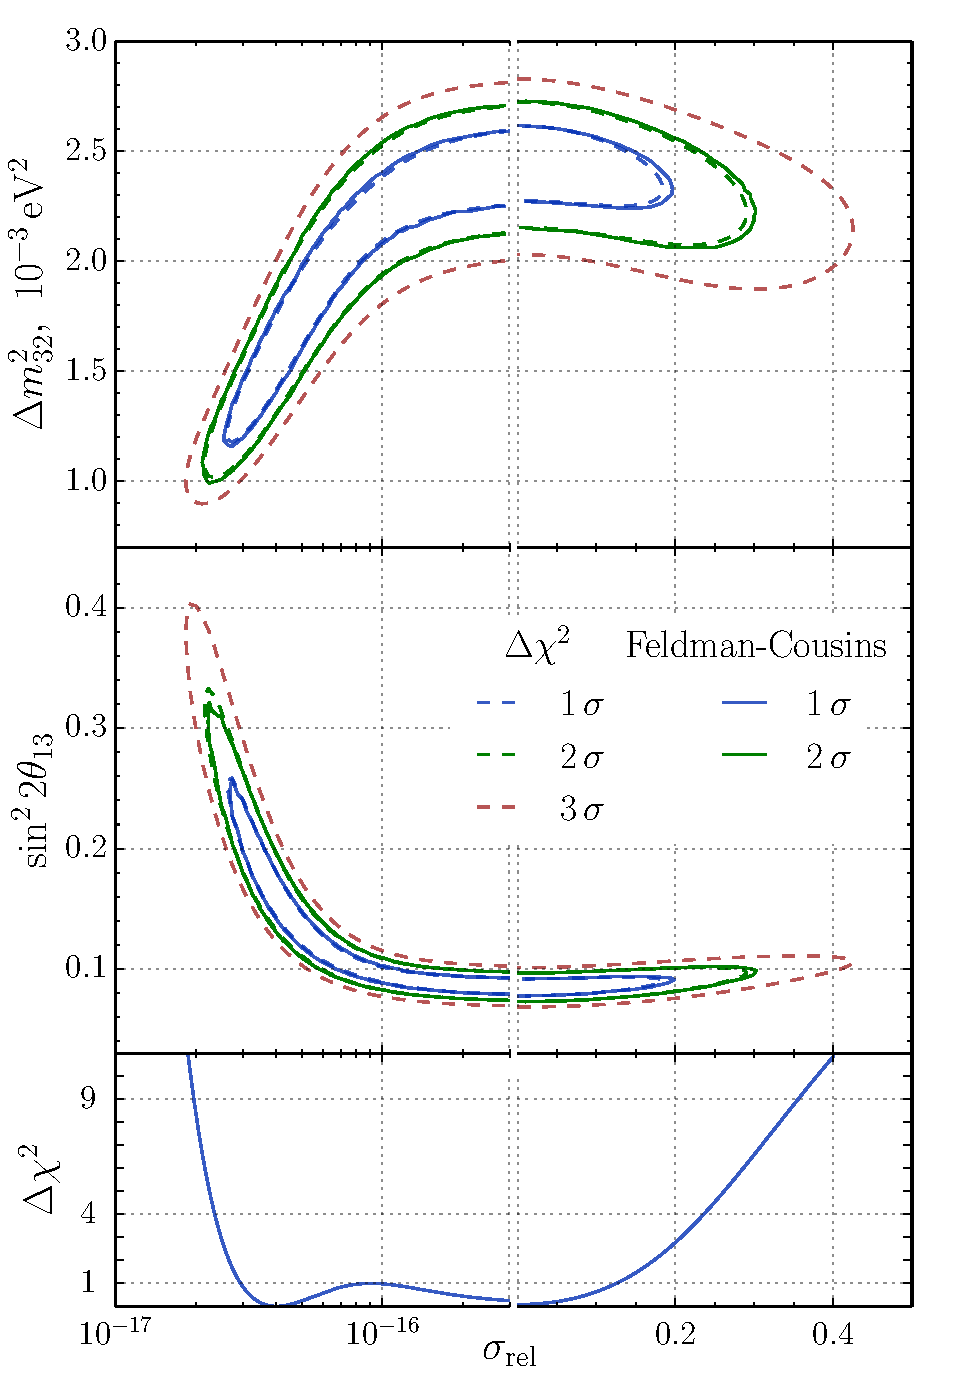
\includegraphics[scale=1.15]{./pics/scan_db_s-dm-th_ihep-fc_v2.pdf}
            \end{figure}
        \end{column}
        \begin{column}{0.57\textwidth}
            \vspace{1cm}
            \begin{itemize}
                \impitem There are 3 distinct regions on \Important{\srel}:
                \vspace*{-1.5cm}
                \begin{itemize}
                    \item \Important{$\srel < 10^{-16}$} -- oscillations are suppresses
                    by \ensuremath{\text{D}^2}.
                    \item \Important{$10^{-16} < \srel < 0.1$} -- no impact on
                    oscillations.
                    \item \Important{$\srel > 0.1$} -- loss of coherence
                    due to spacial separation
                    \Important{\Lcoh} and dispersion \Important{\Ld}.
                \end{itemize}
                \impitem Allowed region for \srel\, at 95\%~C.L.:
                \begin{center}
                    \colorbox{OliveGreen!20}{\raisebox{0}[1.2\height]{\makebox[13em][c]{
                    \begin{equation*}
                        2.38 \cdot 10^{-17} < \srel < 0.232
                    \end{equation*}
                    }}}
                \end{center}
                \impitem The lower limit is weeker than constrains from reactor cores and detector
                dimensions. Combined limits are:
                \begin{center}
                    \colorbox{OliveGreen!20}{\raisebox{0}[1.2\height]{\makebox[13em][c]{
                    \begin{equation*}
                        10^{-11}\, \text{cm} \lesssim \six \lesssim 2\, \text{m}
                    \end{equation*}
                    }}}
                \end{center}
                \impitem The upper limit on \srel\, is
                \begin{center}
                    \colorbox{OliveGreen!20}{\raisebox{0}[1.2\height]{\makebox[13em]{\srel <
                        0.2 at 95\% C.L.}}}
                \end{center}
            \end{itemize}
        \end{column}
    \end{columns}
\end{block}

\vspace{.3cm}
\begin{block}{Conclusion}
    \begin{itemize}
        \impitem First experimental limits on \Important{\srel{}} are obtained.
        \impitem Insignificance of decoherence effect ensures unbiased measurent of oscillation
        parameters within standard approach.
    \end{itemize}
\end{block}

\end{column}

\end{columns}

\end{frame}
\end{document}
